\chapter{MODELO DO REFLETOR CIRCULAR E O MÉTODO ERC}
\label{cap7}

Uma maneira bastante didática de entender o empilhamento SRC é partir de um modelo simples,
derivar a superfície de tempo de trânsito SRC em função dos
parâmetros da geometria do modelo:
No caso do modelo do refletor circular,  representado esquematicamente na Figura \ref{fig:7.1}, 
em um meio homogêneo de velocidade $v_0$,
a solução analítica fechada é complicada, pois envolve uma solução de uma equação polinomial de
alta ordem \cite{landa}.
No entanto, a superfície de tempo de trânsito de reflexão pode ser descrita analiticamente por relações paramétricas
\cite{glaeser}.

%figura da hipérbole
\begin{figure}[htb]
\caption{Representação esquemática do modelo do refletor circular de profundidade $D$
em um meio de velocidade constante $v_0$.
$m$ é a posição do ponto médio do par fonte $s$ e receptor $r$, $L=R+D$ é o comprimento do raio normal, 
$\beta_0$ é ângulo de emergência
do raio normal na superfície e $R$ é o raio do refletor circular.}
\begin{flushleft}
\includegraphics[scale=0.45]{circ.png}
\vspace{-0.3cm}
\end{flushleft}
\begin{center}
 Fonte: Do Autor.
\end{center}
\label{fig:7.1}
\end{figure}



As coordenadas do ponto médio $m$ e do meio-afastamento $h=x/2$ 
são expressas paramétricamente por:

\begin{equation}
\label{eq:7.1}
 m=R\sin(\gamma)+(D+R-R\cos(\gamma))\frac{\cos(\gamma)\cos(\gamma)}{\cos^2(\theta)-\sin^2(\gamma)}
\end{equation}

\begin{equation}
\label{eq:7.2}
 h=(D+R-R\cos(\gamma))\frac{\cos(\theta)\cos(\theta)}{\cos^2(\theta)-\sin^2(\gamma)}
\end{equation}

\begin{figure}[htb]
\caption{Representação esquemática de um arranjo ERC }
\begin{center}
\includegraphics[scale=0.5]{coordenadas.png}
\vspace{-0.3cm}
\end{center}
\begin{center}
 Fonte: Do Autor.
\end{center}
\label{fig:7.2}
\end{figure}


E o tempo de reflexão é expresso como:

\begin{equation}
\begin{flalign*}
\label{eq:7.3}
 \Psi &=\frac{D+R-R\cos(\gamma)}{v_0} \left[ \frac{1}{\cos(\gamma-\theta)}+\frac{1}{\cos(\gamma+\theta)} \right] \\
 &=2\frac{D+R-R\cos(\gamma)}{v_0}\frac{\cos(\gamma)\cos(\theta)}{\cos^2(\theta)-\sin^2(\gamma)}
\end{flalign*} 
\end{equation}


\begin{figure}[htb]
\caption{Representação esquemática do modelo do refletor circular de profundidade $D$
em um meio de velocidade constante $v_0$.
$m$ é a posição do ponto médio do par fonte $s$ e receptor $r$, $L=R+D$ é o comprimento do raio normal, 
$\beta_0$ é ângulo de emergência
do raio normal na superfície e $R$ é o raio do refletor circular.}
\begin{flushleft}
\includegraphics[scale=0.45]{circ_mod.png}
\vspace{-0.3cm}
\end{flushleft}
\begin{center}
 Fonte: Do Autor.
\end{center}
\label{fig:7.3}
\end{figure}

Analisnado a Figura \ref{fig:7.1} podemos ver que os parâmetros do SRC podem ser obtidos a partir
de relações trigonométricas simples apliacadas ao triâmgulo retângulo da Figura \ref{fig:7.3}, de cateto menor
$m_0$, cateto maior $L=D+R$ e hipotenusa $R_N=R+R_{NIP}$.
A relação com os parâmetros do SRC é dada analiticamente, em função dos parâmetros do modelo, por:

\begin{equation}
\label{eq:7.4}
t_0=\frac{2(\sqrt{m_0^2+L^2}-R)}{v_0}
\end{equation}

\begin{equation}
\label{eq:7.5}
R_{NIP}=\sqrt{m_0^2+L^2}-R
\end{equation}

\begin{equation}
\label{eq:7.6}
R_N =\sqrt{m_0^2+L^2}
\end{equation}

\begin{equation}
\label{eq:7.7}
\sin(\beta_0)=\frac{m_0}{\sqrt{m_0^2+L^2}}
\end{equation}


As Equações \ref{eq:7.1}-\ref{eq:7.3} definem a superfície de tempo de reflexão $\Psi(h,d)$ pela dependência paramétrica
$\{m(\alpha,\theta),h(\alpha,\theta),\Psi(\alpha,\theta)\}$.
Onde $L=D+R$, $v_0$ é a velocidade do meio, $\beta_0$ é ângulo de emergência
do raio normal, e $m_0$ é o ponto médio central.


\section{ELEMENTO DE REFLEXÃO COMUM (ERC)}

O método do elemento de reflexão comum (CRE) é uma alternativa interessante para os métodos usuais de empilhamento PMC ou
migração para a seção de afastamento nulo. No entanto não requere conhecimento do modelo geral em subsuperfície, apenas
o conhecimento da velocidade próximo a superfície é necessário a priori.
O método ERC é baseado somente em considerações cinemáticas em 2D e não é
um processo que preserva as amplitudes.

A principal e provavelmente mais importante vantagem do método ERC em comparação com o empilhamento PMC convencional
é que este proporciona, além da seção empilhada, parâmetros importantes para a construção do macromodelo de 
velocidades que pode inclusive variar lateralmente.
Estes parâmetros são atributos específicos de uma frente de onda hipotética atribuídos a cada evento de reflexão
primária de afastamento nulo: O raio de curvatura RNIP e o ângulo de emergência $\beta_0$. Esta onda hipotética é
a onda NIP \cite{hubral}.
Os parâmetros $R_{NIP}$ e $\beta_0$ atribuídos aos pontos $P_0(x_0,\tau_0)$ são obtidos a partir do método ERC.
Estes dois atributos podem ser utilizados para estimar o macromodelo de velocidades.
O método ERC, além de ser um processo para simular as seções de afastamento nulo sem o conhecimento prévio
do macromodelo de velocidades, também permite determinar os atributos da onda NIP $(R_{NIP},\beta_0)$
que combinado com outras estratégias permitem estimar o macromodelo de velocidades.

As principais características do método ERC:
(a) A construção da seção de afastamento nulo a partir de um conjunto de seções de afastamento constante
com apenas uma estimativa da velocidade próxima da superfície.
(b) A determinação dos parâmetros $(R_{NIP},\beta_0)$ para as reflexões de afastamento nulo na seção empilhada.
Estes atributos podem ser utilizados com técnicas de inversão para estimar o macromodelo de velocidades.

A idéia principal do método ERC é, usando a fórmula do tempo de trânsito ERC, no modelo auxiliar, dado um intervalo
de busca para os parâmetros $R_{NIP}$ e $\beta_0$, encontrar a frente de onda NIP que melhor se ajusta aos dados.
Este processo é semelhante a análise sobretempo normal convencional, todavia enquanto esta análise é feita no
domínio PMC, o método ERC é feito no domínio ERC construído durante o processo, o parâmetro otimizado $R_{NIP}$,$\beta_0$
é especificado a partir da análise de coerência nos dados.


\begin{figure}[htb]
\caption{Representação esquemática de um arranjo ERC para um refletor circular de raio $R$ e profundidade
mínima $D$: A família ERC é formada pelos pares $s_i$-$r_i$ (fonte-receptor) que possuem o mesmo ponto de
reflexão em subsuperfície ($NIP$). A família ERC pode ser entendida a partir de uma fonte pontual explosiva
no ponto $NIP$, que ao ser ativada forma uma frente de onda $NIP$ que atinge a superfície em um PMC central 
$m_0$ com raio de curvatura $R_{NIP}$ e ângulo de incidência $\beta_0$.}
\begin{center}
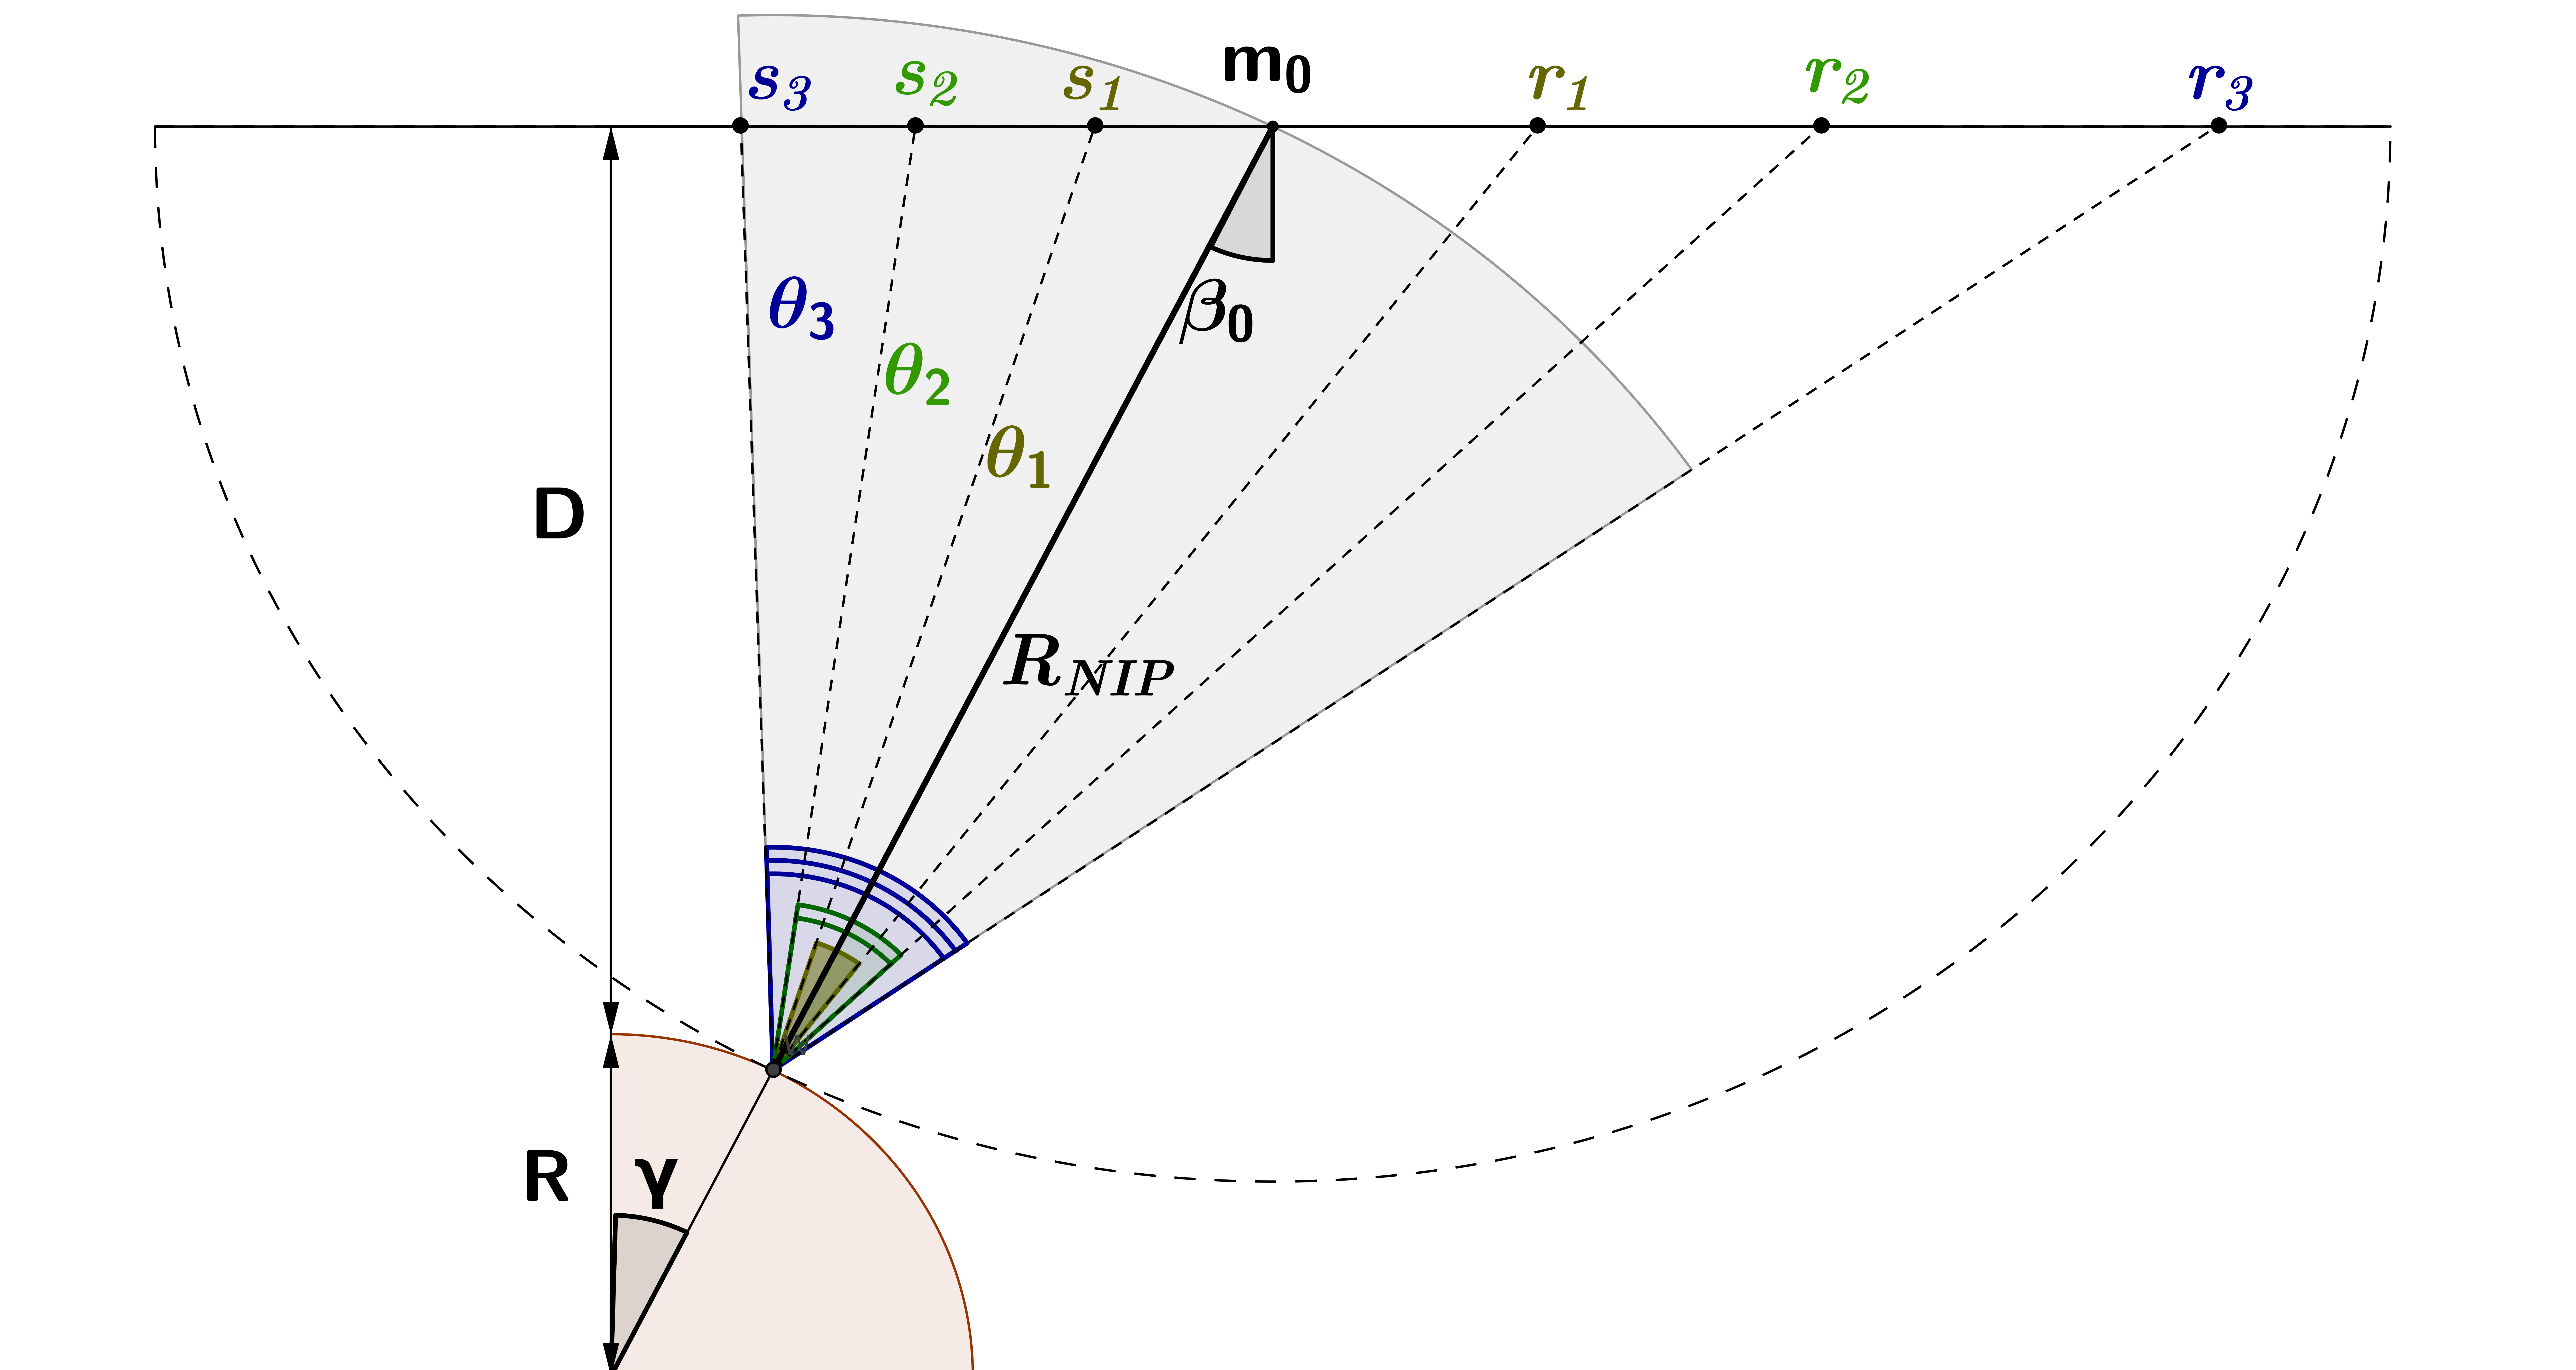
\includegraphics[scale=0.4]{cre.png}
\vspace{-0.3cm}
\end{center}
\begin{center}
 Fonte: Do Autor.
\end{center}
\label{fig:4.1}
\end{figure}


\begin{figure}[htb]
\caption{Representação esquemática das coordenadas do ERC sobre o modelo do refletor circular da Figura \ref{fig:4.1}:
Modificamos a posição do PMC central $m_0$ variando o ângulo $\gamma$ no modelo do refletor circular.
Ao variarmos o ângulo $\theta$, mantendo $\gamma$ constante, obtemos os pares $s_i$-$r_i$ (fonte-receptor)
dentro da família
ERC, as posições $h$ (meio afastamento) e $m$ (PMC) são obtidas para cada par fonte-receptor.
Cada curva colorida representa uma posição
diferente de $m_0$, um valor diferente de $R_{NIP}$ e $\beta_0$, e uma família ERC diferente.}
\begin{center}
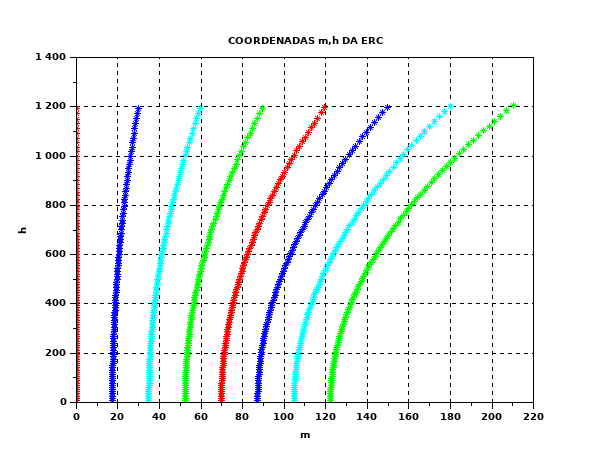
\includegraphics[scale=0.5]{coordenadas_CRE.png}
\vspace{-0.3cm}
\end{center}
\begin{center}
 Fonte: Do Autor.
\end{center}
\label{fig:4.2}
\end{figure}





O parâmetro de assimetria desenpenha um papel importante na seleção de pares fonte-receptor para os quais
o correspondente raio de reflexão refletem no mesmo ponto \cite{tygel}.




